\section{Pre-process}
To make the algorithm faster, could be interesting to do a pre-processing of the data.
Vary approaches were tested, all of them involving the quantities defined in~\ref{ch:structure}. The goal is to identify components which are able to best separate the realisations. 
\paragraph{Low occurrence genes} were selected firstly to make topic modelling. A  $0.5$ threshold was set. This method select genes that appears (have expression greater than zero) only in less than half samples. This doesn't consider genes that appear everywhere (with occurrence $\simeq 1$) but changes their behaviour across realisations.

\paragraph{tf-idf (term frequency–inverse document frequency)} should help. This approach doesn't consider values, but a transformed version
\[
n^{new}_{ij}=\frac{n_{i j}}{M_j}\times \left(1-Log\left(o_i\right)\right)
\] which increases the importance of components with small occurrence $o_i$. This approach doesn't actually select components, which is still an issue.

\paragraph{Highly variable} genes can be selected. This is done using the $CV^2$ analysis from \draft{metti referenza giusta}.
\begin{figure}[htb!]
    \centering
    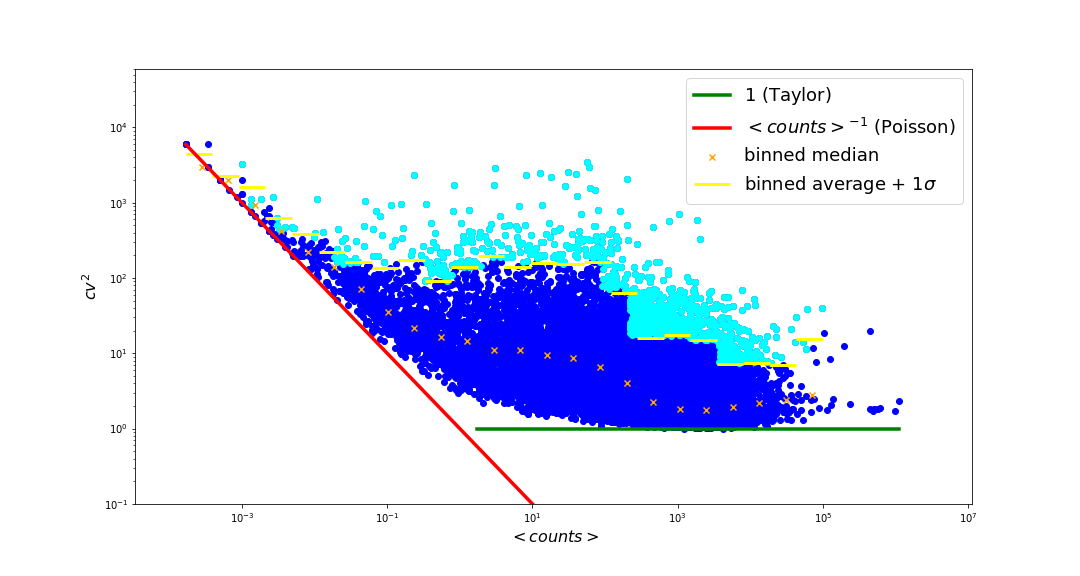
\includegraphics[width=0.8\linewidth]{pictures/topic/cvmean_oversigma.png}
    \caption{Highly variable genes}
    \label{fig:topic/cvmean_oversigma}
\end{figure}
Plotting the coefficient of variation versus the mean for each component reveals which components have higher variance with respect to components which, on average, have a similar behaviour.
Binned averages and variances were estimated, and only genes with a $CV^2$ over a $\sigma$ greater than the bin's mean were considered.

\paragraph{Distance from boundaries} can be a similar and alternative method to select highly variable genes.
\draft{metti figura giusta!!}
\begin{figure}[htb!]
    \centering
    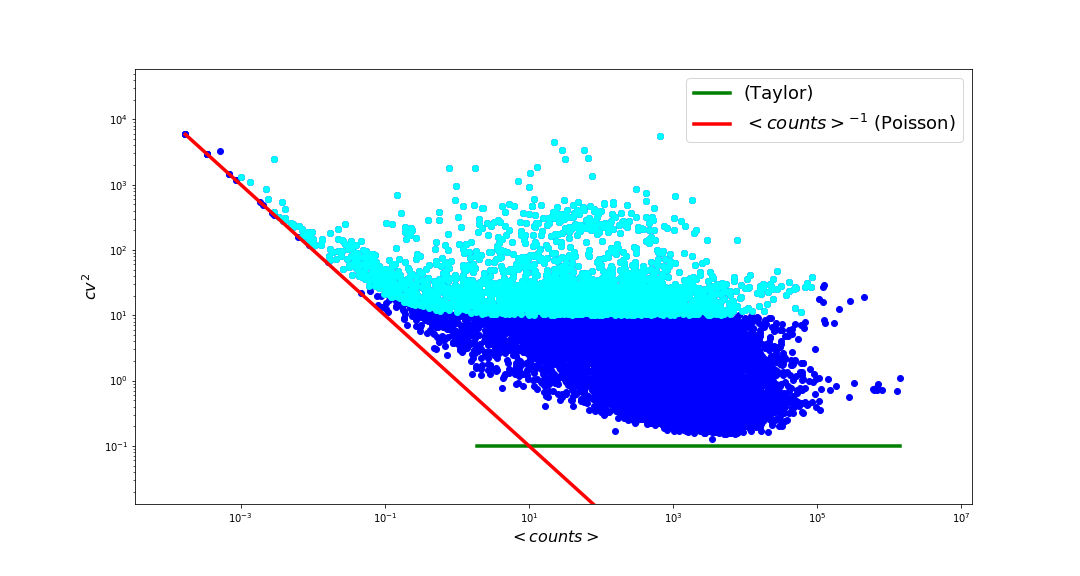
\includegraphics[width=0.8\linewidth]{pictures/topic/cvmean_oversampling.png}
    \caption{Genes distant from the boundaries}
    \label{fig:topic/cvmean_oversampling}
\end{figure}
The distribution as discussed in \draft{disctuti e linka} have a Poisson-like and a Taylor-like boundaries. So can be considered only components that are the most distant from these boundaries.

Using the last two approaches got the point and actually help topic modelling to succeed.